%%%%%%%%%%%%%%%%%%%%%%%%%%%%%%%%%%%%%%%%%%%%%%%%%%%%%%%%%%%%%%%%%%%%%%%%%%%%%%%%%%%%%%%%%%

\section*{Задание}
Написать курсовую/диплом/отчет и разобраться в работе \LaTeX\ .
\addcontentsline{toc}{section}{Задание}

\section*{Как быстро начать работу с шаблоном}
\addcontentsline{toc}{section}{Как быстро начать работу с шаблоном}
Если вы хотите быстро начать, нужно: 
\begin{enumerate}
\item зайти в main.tex и удалить/закомментировать строку с \textbf{include\{tutorial\}}.
\image{tutor1.png}{include tutorial}{0.7}
\item загрузить свой титульный лист в формате pdf и назвать его titlepage, либо есть титульный лист не нужен удалить/закомментировать строку с includepdf.
\image{tutor2.png}{include titlepage.pdf}{0.7}
\item Открываете \textbf{content.tex} и начинаете работу над отчётом.
\end{enumerate}

На этом все, далее вам будет доступны ещё две страницы - содержание и источники. Содержание будет редактироваться автоматически, источники можно либо убрать, либо в файле refs.bib указать их.



\section*{Начало работы}
\addcontentsline{toc}{section}{Начало работы}

Итак, вы скачали этот шаблон (за что вам огромное спасибо), но совершенно не разбираетесь как работать с \LaTeX, что же делать? Давайте разбираться.


\section{Структура шаблона}
Самый важный файл в шаблоне - \textbf{main.tex}. Его нельзя удалять, изменять нужно с осторожностью. Именно он является главным исполняемым файлом, в него включаются все остальные \textbf{.tex }файлы и библиография.



Шаблон имеет 3 папки - \textbf{Images}, \textbf{Listings}, \textbf{Settings}. 
\begin{itemize}
\item В папке \textbf{Images} содержаться изображения, которые войдут в документ. Если вам нужно вставить изображение - прежде всего загрузите его сюда.
\item В папке \textbf{Listings} содержатся файлы с кодом, которые специальной командой можно быстро вставить в документ в качестве листинга.
\item В папке \textbf{Settings} содержатся технические \textbf{.tex} файлы с настройками. Поскольку их довольно много, чтобы не мозолить глаза они были перемещены сюда.
\end{itemize}
В папке Settings содержатся два важных .tex файла - \textbf{packages }и \textbf{format}. Первый отвечает за все пакеты нужные для работы шаблона, второй за формат текста, шрифты, изображения и многие другие вещи.

Если вам нужно добавить какие-то фичи или же изменить положение текста, шрифт и тд - меняйте эти файлы под себя.

Далее идут два опциональных .tex файла - tocpage и bibpage. Страница Содержания и страница Источников. Эти страницы отделены поскольку они не всегда нужны, поэтому чтобы не загромождать шаблон были вынесены в отдельные файлы.

Никто не мешает вам убрать их и вводить как Содержание, так источники вручную.

Свой отчет нужно вводить в файл \textbf{content.tex}.


%%%%%%%%%%%%%%%%%%%%%%%%%%%%%%%%%%%%%%%%%%%%%%%%%%%%%%%%%%%%%%%%%%%%
\section{Как писать символы}
Чтобы не возникло проблем сразу обрисую ситуацию - на LaTeX нельзя просто вводить символы, которые используются в языке Tex. Это символы:

\begin{minted}{text}
$ & % # _ { } ~ ^ \
\end{minted}
Чтобы использовать их обязательно нужно вводить их так:
\begin{minted}{text}
\$ \& \% \# \_ \{ \} \~ \^
\end{minted}
Это касается и обычного текста, и названий заголовков.








%%%%%%%%%%%%%%%%%%%%%%%%%%%%%%%%%%%%%%%%%%%%%%%%%%%%%%%%%%%%%%%%%%%%
\section{Как писать текст}
Писать текст очень легко. Все новые абзацы начинаются с красной строки. Размер текста и поля по краям по ГОСТ'у. \\Можно начать с новой строки используя двойную косую черту.

А начать новый абзац можно отступив одну строку между текстом.

\textit{...социально-экономическое развитие требует от нас анализа экономической целесообразности принимаемых решений?} \cite{kistyakovskii} 

Также можно цитировать командой \textbf{cite}.

Чтобы добавлять заголовки - воспользуйтесь командой \textbf{section}, подзаголовки - \textbf{subsection}. Они сразу добавятся в Содержание. 

Если вам нужно добавить заголовок или подзаголовок без нумерации - добавьте в конце \textbf{*}. Чтобы они появились в Содержании воспользуйтесь \textbf{addcontentsline} как это показанато тут.


\begin{minted}{Tex}
\section*{Начало работы}
\addcontentsline{toc}{section}{Начало работы}
\end{minted}

В итоге получится полностью рабочий заголовок в содержании.

%%%%%%%%%%%%%%%%%%%%%%%%%%%%%%%%%%%%%%%%%%%%%%%%%%%%%%%%%%%%%%%%%%%%
\section{Как вставлять рисунки}


Можно вручную вставлять рисунки прописывая каждый параметр:

\begin{minted} {Tex}
\begin{figure}[!htb]
    \centering
    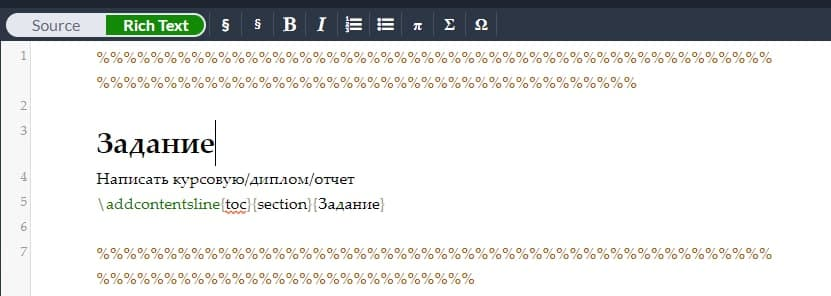
\includegraphics[width=\textwidth]{image1.jpg}
    \caption{Используйте Rich Text}
    \label{fig:image1}
\end{figure}
\end{minted}


\begin{figure}[!htb]
	\centering
	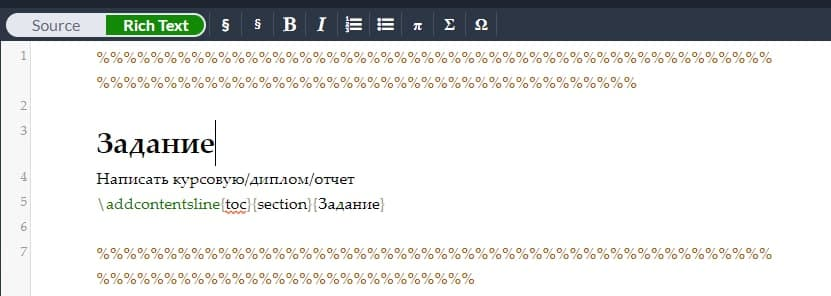
\includegraphics[width=\textwidth]{image1.jpg}
	\caption{Используйте Rich Text}
	\label{fig:image1}
\end{figure}

Параметр \textbf{width} задаёт ширину рисунка. В этом случае она равна ширине текста \textbf{(textwidth}). Перед\textbf{ textwidth} можно указать значение от 0.1 до 1.
А можно использовать кастомную команду image:
\begin{minted} {Tex}
\image{image2.jpg}{Подпись к рисунку}{0.7}
\end{minted}

\image{image2.jpg}{Подпись к рисунку}{0.7}

Она позволяет удобно и быстро вставлять и регулировать размер изображения, для того чтобы исключить проблемы с разметкой изображений на странице. Размер можно менять изменяя второй параметр, который принимает любое число с плавающей точкой, но я рекомендую использовать лишь в диапазоне от 0.1 до 1, поскольку команда автоматически скейлит маленькое изображение, а с большими могут возникать проблемы.
\newpage
\begin{minted} {Tex}
\image{image2.jpg}{То же изображение, но меньше}{0.35}
\end{minted}

\image{image2.jpg}{То же изображение, но меньше}{0.35}

К тому же команда автоматически проставляет нумерацию рисунков.
\section{Как вставлять таблицы}
К сожалению таблицы это комплексная вещь, поэтому придется задавать все параметры вручную.

Однако очень рекомендую \href{https://truben.no/table/}{этот сайт}, тут можно очень легко делать таблицы и потом вставлять сгенерированный код в свой документ.
\image{tableeditor.png}{Table Editor}{0.8}
\newpage
\begin{minted} {Tex}
\begin{table}[h!]
\centering
\begin{tabular}{|c|c|c|c|} 
    \hline
    Столбец1 & Столбец2 & Столбец3 & Столбец4 \\ [0.5ex] 
        \hline
        \multirow{3}{5em}{Несколько строк} & 6 & 87837 & 787 \\ 
        &  7 & 78 & 5415 \\
        & 545 & 778 & 7507 \\
        & 545 & 18744 & 7560 \\
        & 88 & 788 & 6344 \\ [1ex] 
 \hline
\end{tabular}
\caption{Пример работы с таблицей}
\label{table:1}
\end{table}
\end{minted}




Вот пример таблицы:

\begin{table}[h!]
\centering
\begin{tabular}{|c|c|c|c|} 
    \hline
    Столбец1 & Столбец2 & Столбец3 & Столбец4 \\ [0.5ex] 
        \hline
        \multirow{3}{5em}{Несколько строк} & 6 & 87837 & 787 \\ 
        &  7 & 78 & 5415 \\
        & 545 & 778 & 7507 \\
        & 545 & 18744 & 7560 \\
        & 88 & 788 & 6344 \\ [1ex] 
    \hline
\end{tabular}
\caption{Пример работы с таблицей}
\label{table:1}
\end{table}


Больше о таблицах \href{https://www.overleaf.com/learn/latex/Tables}{тут}.

%%%%%%%%%%%%%%%%%%%%%%%%%%%%%%%%%%%%%%%%%%%%%%%%%%%%%%%%%%%%%%%%%%%%
\section{Как работать с математикой}

    \subsection{Математические формулы}
    Хорошо известная теорема Пифагора \(x^2 + y^2 = z^2\) была
    доказана недействительной для других показателей.
    Это означает, что следующее уравнение не имеет целочисленных решений:
    \[ x^n + y^n = z^n \]
    Другой способ вставить уравнение в текст такой: $x^2 + y^2 = z^2$. То есть уравнение нужно поместить между двумя знаками "доллара".

    \subsection{Дроби}
    При отображении дробей в строке, например \(\frac{3x}{2}\),
    вы можете установить другой стиль отображения:
    \( \displaystyle \frac{3x}{2} \).
    Это также верно и в обратном направлении
    \[ f(x)=\frac{P(x)}{Q(x)} \ \ \textrm{и}
    \ \ f(x)=\textstyle\frac{P(x)}{Q(x)} \]

    \subsection{Интегралы}
    Интеграл \(\int_{a}^{b} x^2 dx\) внутри текста.
    \medskip
    Тот же интеграл на дисплее:
    \[
    \int_{a}^{b} x^2 \,dx
    \]
    Официальнный туториал по интегралам можно посмотреть по этой  \href{https://www.overleaf.com/learn/latex/Integrals,_sums_and_limits#Integrals}{ссылке}.

    \subsection{Сумма и произведение}
    Тоже оставлю \href{https://www.overleaf.com/learn/latex/Integrals,_sums_and_limits#Sums_and_products}{ссылку}.
    
    \subsection{Пределы}
    
    Предел \(\lim_{x\to\infty} f(x)\) внутри текста.
    Тот же предел на дисплее:
    \[
    \lim_{x\to\infty} f(x)
    \]

%%%%%%%%%%%%%%%%%%%%%%%%%%%%%%%%%%%%%%%%%%%%%%%%%%%%%%%%%%%%%%%%%%%%
\section{Как вставлять листинг кода}




Для листинга можно воспользоваться командой codefromfile.Эта команда позволяет указать файл и вставить его в документ. Может пригодиться если лень копировать и вставлять огромный код. Для того чтобы файл открывался - нужно поместить его в папку Listings.

%\insertcode{Main.java}{Пример кода}
\subsection*{Файл main.java}


% \codefromfile {Имя файла} {Язык Программирования}


\codefromfile{Main.java}{text}

\newpage
Можно воспользоваться командой codefromfile, а можно забить код вручную через среду minted:

\subsection*{Файл def.py}
\begin{minted}
[
frame=lines,
framesep=2mm,
baselinestretch=1.2,
fontsize=\footnotesize,
linenos
]
{text}
import numpy as np
    
def incmatrix(genl1,genl2):
    m = len(genl1)
    n = len(genl2)
    M = None #to become the incidence matrix
    VT = np.zeros((n*m,1), int)  #dummy variable
    
    #compute the bitwise xor matrix
    M1 = bitxormatrix(genl1)
    M2 = np.triu(bitxormatrix(genl2),1) 

    for i in range(m-1):
        for j in range(i+1, m):
            [r,c] = np.where(M2 == M1[i,j])
            for k in range(len(r)):
                VT[(i)*n + r[k]] = 1;
                VT[(i)*n + c[k]] = 1;
                VT[(j)*n + r[k]] = 1;
                VT[(j)*n + c[k]] = 1;
                
                if M is None:
                    M = np.copy(VT)
                else:
                    M = np.concatenate((M, VT), 1)
                
                VT = np.zeros((n*m,1), int)
    
    return M
\end{minted}

При этом добавив к нему кучу красивого оформления - как в этом листинге. \newline

Обратите внимание, что если во вторых скобках указать вместо text любой другой язык, то код будет подсвечиваться:


\newpage
\begin{minted}
{C++}
// quot_rem.cpp
#include <iostream>
#include <cstdlib>

int main()
{
  using namespace std;

  int a = 0, b = 0; // Целые числа.
  cout << "a = ";
  cin >> a;
  cout << "b = ";
  cin >> b;

  cout << "quotient a:b  = " << a / b << endl;
  cout << "remainder a:b = " << a % b << endl;
  return EXIT_SUCCESS;
}

\end{minted}

В данном случае я указал C++. Тоже самое можно будет сделать если указать в команде codefromfile во второй скобке язык:

\newpage
\codefromfile{main.py}{python}

Помимо команд выше можно воспользоваться \textbf{lstlisting}, которая позволяет более точно настроить параметры листинга а также указать подпись к нему. К тому же она автоматически проставляет нумерацию листингов.

\begin{minted}{tex}
\begin{lstlisting}[language=Java, caption=Кириллица в листинге не имеет подсветки]
class HelloWorldApp {
    public static void main(String[] args) {
        System.out.println("Hello, мир!"); // Коментарий на кириллице
        for (int i = 0; i < 100; ++i) {
            System.out.println(i); // Latin comment
        }
    }
}
\end{lstlisting}
\end{minted}




\begin{lstlisting}[language=Java, caption=Кириллица в листинге не имеет подсветки]
class HelloWorldApp {
    public static void main(String[] args) {
        System.out.println("Hello, мир!"); // Коментарий на кириллице
        for (int i = 0; i < 100; ++i) {
            System.out.println(i); // Latin comment
        }
    }
}
\end{lstlisting}

\begin{lstlisting}[language=SQL, caption=Пример на SQL]
SELECT Orders.OrderID, Customers.CustomerName
FROM Orders
INNER JOIN Customers ON Orders.CustomerID = Customers.CustomerID;
\end{lstlisting}

\begin{lstlisting}[language=haskell, caption=Пример на Haskell]
quicksort :: (Ord a) => [a] -> [a]
quicksort [] = []
quicksort (x:xs) =
  let smallerSorted = quicksort [a | a <- xs, a <= x]
      biggerSorted = quicksort [a | a <- xs, a > x]
  in  smallerSorted ++ [x] ++ biggerSorted
\end{lstlisting}



\lstinputlisting[language=Python, caption=Листинг из файла]{Listings/main.py}




%%%%%%%%%%%%%%%%%%%%%%%%%%%%%%%%%%%%%%%%%%%%%%%%%%%%%%%%%%%%%%%%%%%%
\section{Как вставлять специальные символы}
$\alpha A$ - греческие символы,  $ \lambda; \Lambda$ - физические величины, $\exists; \forall$ - логические символы\\
По этой   \href{https://www.overleaf.com/learn/latex/List_of_Greek_letters_and_math_symbols}{ссылке} можно посмотреть остальные символы. \href{https://www.overleaf.com/learn/latex/Operators}{Здесь} - математические операторы.



%%%%%%%%%%%%%%%%%%%%%%%%%%%%%%%%%%%%%%%%%%%%%%%%%%%%%%%%%%%%%%%%%%%%
\section{Руководство}
\href{https://www.texlive.info/CTAN/info/lshort/russian/lshortru.pdf}{Ссылка} на полное введение в Latex на русском языке.


%%%%%%%%%%%%%%%%%%%%%%%%%%%%%%%%%%%%%%%%%%%%%%%%%%%%%%%%%%%%%%%%%%%%
\newpage
\section{Заключение}
Вот вы и закончили написание курсовой/диплома/отчета на \LaTeX, вы великолепны!


%%%%%%%%%%%%%%%%%%%%%%%%%%%%%%%%%%%%%%%%%%%%%%%%%%%%%%%%%%%%%%%%%%%
